\subsection{Vehicle Trajectory [Andy McClaskey]}
The design of this vehicle was based on a 1500 pounds per square foot (71.82 kPa) constant dynamic pressure trajectory. The trajectory was found by iterating Mach number to make the density given in the dynamic pressure equation match that given by the standard atmosphere function. The altitude and velocity trajectory are shown below in Figure \ref{fig:altVMach} and Figure \ref{fig:velVMach}.

\begin{figure}[H]
\begin{center}
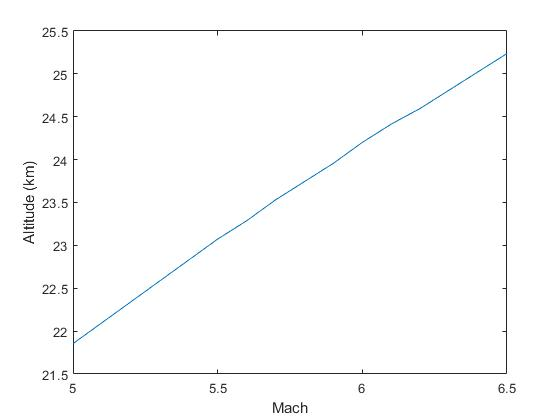
\includegraphics[width=0.6\textwidth]{altVMach}
\caption{Altitude v. Mach}
\label{fig:altVMach}
\end{center}
\end{figure}

\begin{figure}[H]
\begin{center}
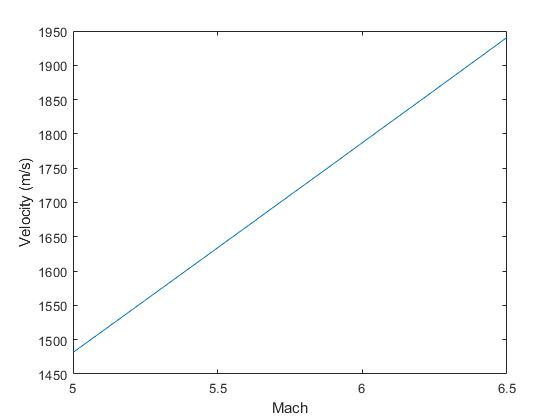
\includegraphics[width=0.6\textwidth]{velVMach}
\caption{Velocity v. Mach}
\label{fig:velVMach}
\end{center}
\end{figure}

The end point shown in Figure \ref{fig:altVMach} and Figure \ref{fig:velVMach} are the cruise conditions for this mission.